\documentclass[12pt,a4paper]{article}

\usepackage{styles/dolgozat}

\usepackage{listings}
% \usepackage{styles/cpp}
\usepackage{styles/python}
\usepackage{indentfirst}

\usepackage{hyperref}

\begin{document}

\pagestyle{empty} %a címlapon ne legyen semmi=empty, azaz nincs fejléc és lábléc

% A Miskolci Egyetem címere
{\large
\begin{center}
\vglue 1truecm
\textbf{\huge\textsc{Beszámoló szakmai gyakorlatról}}\\
\vglue 3truecm

\includegraphics[width=4.8truecm, height=4truecm]{images/me_logo.png}\\
\textbf{\textsc{Miskolci Egyetem}}
\end{center}}

\vglue 1.5truecm %függõleges helykihagyás

% A szakdolgozat címe, akár több sorban is
% A hallgató neve, évfolyam, szak(ok), a konzulens(ek) neve
{\large
\begin{center}
\begin{tabular}{c}
\textbf{Készítette:}\\
Sándor János \\
Programtervező informatikus \\
Neptun kód: \texttt{U03GDK} \\
e-mail cím: \texttt{sandorj2002@gmail.com}
\end{tabular}
\end{center}
\vskip 1cm
\begin{center}
\begin{tabular}{c}
\textbf{Üzemi instruktor:}\\
Piller Imre \\
tanársegéd \\
Alkalmazott Matematikai Intézeti Tanszék, Miskolci Egyetem \\
telefonszám: \texttt{+3646/565-111/14-50}


\end{tabular}
\end{center}}
\vfill
% Keltezés: Hely, év
{\large
\begin{center}
\textbf{\textsc{Miskolc, 2025}}
\end{center}}

\newpage


\newpage

\pagestyle{empty}

\cleardoublepage
\pagenumbering{gobble}
\tableofcontents
\cleardoublepage
\pagenumbering{arabic}

\newpage

\pagestyle{fancy}

\section{A feladat bemutatása}

A \emph{„Túlélés a Szocializmusban”} című játék egy túlélés-orientált szimuláció, amely a szocialista korszak mindennapjainak mindennapi kihívásait, bizonytalanságait és sajátos társadalmi viszonyait dolgozza fel. A projekt elsődleges célja, hogy a játékos interaktív módon tapasztalhassa meg egy olyan rendszer működését, ahol a hétköznapi életet szigorú állami szabályozás, hiánygazdaság és folyamatos alkalmazkodási kényszer határozta meg. A játék így nem pusztán szórakoztatni kíván, hanem gondolkodásra is ösztönöz: a játékosnak újra és újra morális döntéseket kell meghoznia, miközben a túlélés és a hosszabb távú érvényesülés között lavírozik.

A játékmenet egy fiktív, de a történelmi valóság elemeit idéző világban zajlik. A játékos feladata, hogy biztosítsa saját és családja mindennapi megélhetését egy olyan környezetben, ahol a legkisebb döntések is súlyos következményekkel járhatnak. A játék középpontjában a szűkös erőforrások beosztása áll: a munka, a családról való gondoskodás és a személyes szükségletek (például a testi-lelki egészség megőrzése) folyamatos egyensúlyozást igényelnek. A játékmenet változatosságát különféle munkalehetőségek biztosítják – például autószerelő műhelyben végzett precíziós feladatok, bolti eladóként teljesített gyors és pontos kiszolgálás, vagy irodai munka, amely inkább a monotóniatűrést teszi próbára. Mindegyik munkatípus eltérő kihívásokat tartogat, és a játékos teljesítménye közvetlenül kihat bevételeire, valamint reputációjára.

A játék különösen nagy hangsúlyt fektet a társadalmi és gazdasági környezet modellezésére. Az éhség, a stressz, a reputáció és az alkoholfüggőség mutatói folyamatosan változnak a játékos döntései és cselekedetei alapján. Mindezek mellett gondoskodni kell a családtagok jólétéről is, ami tovább fokozza a nyomást és növeli a játékos felelősségét. A korra jellemző hiánygazdaság a játékmenet szerves része: a vásárlás mellett cserekereskedelemre, feketepiaci ügyeskedésre és ismerősökön keresztül történő beszerzésre is lehetőség nyílik, amelyek gyakran morálisan kétséges döntéseket kívánnak meg.

A játékban véletlenszerű események és dilemmák színesítik a mindennapokat, amelyek próbára teszik a játékos erkölcsi érzékét és stratégiai gondolkodását. A könnyebb, de szabálytalan vagy etikailag megkérdőjelezhető megoldások rövid távon előnyt jelenthetnek, azonban hosszabb távon komoly kockázatokat hordoznak: lebukás, reputációvesztés vagy akár a szabadság elvesztése. A legsúlyosabb következmények között szerepelhet a Gulágra való száműzetés, ahol a játék célja teljesen megváltozik: a fejlődés és gyarapodás helyett immár a puszta túlélés válik a központi feladattá.

Összességében a \emph{„Túlélés a Szocializmusban”} nem csupán egy szórakoztató játékként értelmezhető, hanem egy interaktív történelmi élményként is, amely a korszak sajátosságait és dilemmáit a játékos aktív részvételével mutatja be. A projekt elsősorban azon játékosoknak szól, akik nyitottak a történelmi ihletésű, komolyabb hangvételű szimulációs élményekre, és szívesen szembesülnek olyan döntési helyzetekkel, amelyek túlmutatnak a hétköznapi játékmeneten, és valódi társadalmi-történelmi tanulságokat is hordoznak.

A játék külön értéke, hogy nem csupán szimulációs szórakozást nyújt, hanem oktatási és szemléltető funkcióval is bírhat. A fiatalabb generációk számára interaktív módon mutatja be a szocialista korszak társadalmi és gazdasági nehézségeit, miközben a döntési helyzeteken keresztül érzékelteti az egyén kiszolgáltatottságát és a rendszer nyomásait. A projekt így egyszerre szolgálhat történelmi betekintésként, társadalmi gondolkodtatásként és izgalmas játékmenetként, amely egyaránt szólhat a laikus közönséghez és a téma iránt mélyebben érdeklődő játékosokhoz.

\section{Technológia kiválasztása}

A játék fejlesztéséhez a Godot Game Engine került kiválasztásra, amely egy nyílt forráskódú, platformfüggetlen játékmotor. A Godot kiemelkedik a könnyen használható vizuális szerkesztőjével, a különböző 2D és 3D játékmechanikák támogatásával, valamint a beépített scriptelési nyelvével, a GDScript-tel, amely Python-szerű szintaxisával gyors prototípus-készítést tesz lehetővé.

A GDScript hivatalos dokumentációja részletes útmutatót nyújt a nyelv alapjairól, típusairól és a Godot engine-beli integrációról \cite{gdscript_basics,gdscript_learn}. Emellett a GDQuest interaktív tanfolyamai is hasznosak a kezdő fejlesztők számára \cite{gdquest_gdscript}.

A Godot előnyei közé tartozik a kis erőforrásigény, a széleskörű dokumentáció és a folyamatosan fejlődő közösség, amely rengeteg mintaprojektet és bővítményt biztosít. Ezek lehetővé teszik, hogy a játékfejlesztők gyorsan és hatékonyan valósítsák meg a játék mechanikáit, a felhasználói felületet és a vizuális elemeket, miközben a motor teljesen ingyenesen használható, ami különösen előnyös kisebb, hallgatói vagy indie projektek esetén \cite{holfeld2023relevance,salmela2022game}.


\section{A tervezés folyamata}

A projektet négyen fejlesztettük, és mindenki foglalkozott a különböző feladatokkal: programozási részek, grafika, textúrák készítése, dokumentálás és tesztelés. Minden tag hozzájárult a kódoláshoz és a vizuális elemek kialakításához, így a munkamegosztás rugalmas volt és a csapat minden tagja több területen is részt vett.

Emellett én láttam el a projektmenedzseri feladatokat is, azaz koordináltam a csapat munkáját, felosztottam a feladatokat, kapcsolatot tartottam a gyakorlatvezetővel, nyomon követtem a határidőket és biztosítottam, hogy minden részfeladat összehangoltan haladjon.  

\subsection{Előkészületek}

A projekt kezdetén átbeszéltem a csapattal a projektstruktúrát, és közösen megbeszéltük a játék főbb elemeit, a feladatokat és a határidőket. Elkészítettem a fejlesztési tervet, meghatároztam a játék leírását, valamint összeszerveztem a csapatot, hogy minden tag tudja, milyen területen dolgozik, és a munka összehangoltan haladjon.  
Egy kisebb rész az általam írt fejlesztési tervből:

\textbf{Analízis modell megalapozása:}
\begin{itemize}
    \item Megbeszélés az analízis modellbe kerülő elemekről, úgy mint use case diagram, osztálydiagram, állapotdiagram. Az így elkészített osztálydiagramok \aref{fig:classdia} ábrán láthatók.
    \item Alap játékmeneti ciklus és események rendszerezése (pl. reggel → munka → este → pihenés).
    \item A játéklogika és történet szorosabb integrációja: játékos feladatai, célok, morális döntések helye és szerepe.
\end{itemize}
\Aref{tab:project_schedule} táblázat összesíti az egyes előkészületeket.
\begin{table}[h!]
\centering
\caption{Projekt ütemezés és heti feladatok}
\label{tab:project_schedule}
\begin{tabular}{|c|c|p{8cm}|c|}
\hline
\textbf{Hét} & \textbf{Konzultációs Napok} & \textbf{Fő tevékenységek} \\ \hline
1–2. & Kedd, Péntek, Vasárnap & Játékkoncepció véglegesítése, alap játékmenet, projektstruktúra kialakítása, Git/GitHub beállítások \\ \hline
3–4. & Kedd, Péntek, Vasárnap & Grafikai koncepciók kidolgozása\aref{fig:office}, analízis modell (use case, osztálydiagram)\aref{fig:classdia}, HUD és menütervezés \\ \hline
5–6. & Kedd, Péntek, Vasárnap & Rendszerterv véglegesítése, moduláris script rendszer kialakítása, prototípus elkészítése \\ \hline
7–8. & Kedd, Péntek, Vasárnap & Funkciók finomhangolása, tesztelés, UI és grafikai polish, végső dokumentáció és build készítése  \\ \hline
\end{tabular}
\end{table}


\subsection{Projektmenedzselés}

A projekt során a konzultációk koordinálása és a csapattagok feladatainak elosztása is az én feladatom volt. Minden konzultációra, különösen a vasárnapi megbeszélésekre előre felkészültem: előkészítettem a feladatcsomagokat, így a csapattagoknak már csak a négy részre osztott feladatok közül kellett választaniuk. A feladatokat egyenletesen osztottam el típusonként, biztosítva, hogy mindenki részt vehessen a projekt különböző területein, beleértve a grafikai, kódolási, tesztelési és dokumentációs feladatokat.  

Folyamatosan tartottam a kapcsolatot a gyakorlatvezetővel, reagálva minden tanácsára és észrevételére, és segítettem a projekt gördülékeny működését. Egy személyes konzultációt is lebonyolítottunk a gyakorlatvezetővel, amely során részletesen átbeszéltük a projekt állását és a következő lépéseket.  

Emellett a GitHub repository kezelése is a feladatom volt: bemutattam a branch-ek használatát a csapattagoknak, létrehoztam az összes issue-t, hozzárendeltem a felelősöket és típusokat, valamint koordináltam az összes pull request feldolgozását. A folyamat a projekt elején még nehézkes volt, de a végére hatékonyan és gördülékenyen működött.  

Összefoglalva, a projektmenedzselés során magabiztos tapasztalatokat szereztem a kisebb csapat irányításában, a rugalmas támogatásban, az eszközök karbantartásában, valamint az agilis módszertanok alkalmazásában, melyet Piller Imre is ajánlott számomra.

\subsection{Dokumentálás}

A projekt során a dokumentációs feladatok koordinálása és a dokumentumok előkészítése, kidolgozása szintén a feladatom volt. A kezdeti szakaszban a projekt struktúráját, a fejlesztési tervet és a tájékoztató dokumentumot dolgoztam ki és illesztettem bele a projekttervbe. A vízió felosztását közösen végeztük el, míg a bevezetés, áttekintés, problémamegoldás, játéktörténet, játékmechanika és a játékmenet kidolgozása dokumentációs feladatként a részem volt. Az SRS dokumentum részeit – „Játéktörténet”, „Játékmechanika”, „Játékmenet” és „Játéklogika” – összesítettem és összehangoltam, biztosítva az egységes stílust és a megfelelő tartalmi összefüggéseket.

Az analízis modell elkészítése során részt vettem az osztálydiagramok, alrendszerek és menüalrendszerek kidolgozásában, valamint a pull requestek origin/main-hoz történő kezelésében. A fejlesztési terv különböző heti szakaszait részletesen dokumentáltam, beleértve a Gantt-diagramok létrehozását és a feladatok elosztását a csapattagok között. A diagramok Visual Paradigm \cite{visualparadigm_online} online szerkesztőeszközzel készültek.

\begin{figure}[h]
    \centering
    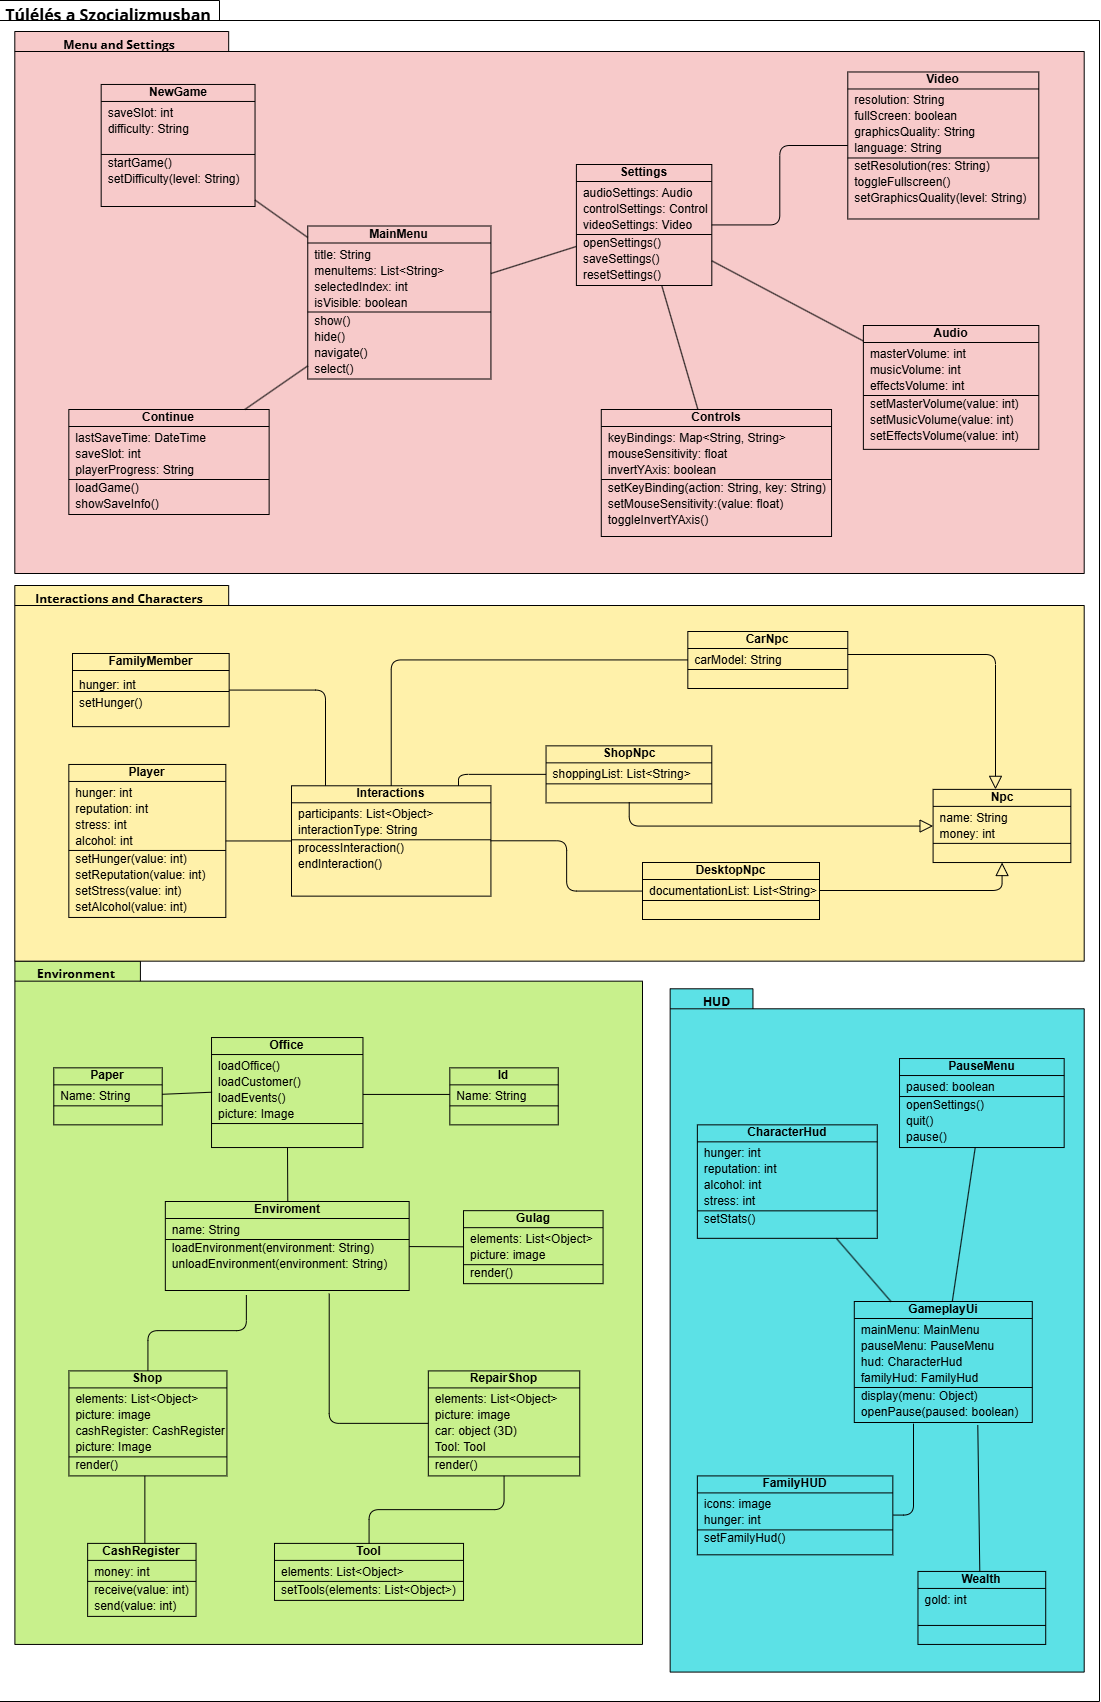
\includegraphics[width=0.6\textwidth]{latex/images/classdiagram.png}
    \caption{Általam elkészített osztálydiagram.}
    \label{fig:classdia}
\end{figure}

Emellett a Godot projekt struktúráját, a scenes és import elemek kezelését dokumentáltam, segítettem a textúrák hozzáadásában és finomításában, valamint a hibák visszafordításában és javításában. A fejlesztési terv véglegesítéséig folyamatosan frissítettem a dokumentációt, rögzítve az elvárt eredményeket, a grafikai és technikai elemek állapotát, valamint az analízis modell részleteit.

Összességében a dokumentálási tevékenységek során a projekt teljes időszakában biztosítottam a dokumentumok naprakészségét, az egységes szerkezetet és a csapat minden tagja számára világos eligazítást a feladatok végrehajtásához.

\section{Implementáció}

A fejlesztés során a játék fő komponenseit a Godot Engine segítségével valósítottuk meg. 
A projekt struktúráját és a scripteket modulárisan szerveztük, biztosítva a különböző játékmechanikák, 
grafikai elemek és kezelőfelületi részek egyszerű integrálását. Az implementáció során 
a csapat minden tagja részt vett a grafikai és logikai modulok fejlesztésében, 
miközben a projektmenedzser koordinálta a feladatok kiosztását, a verziókezelést és a belső tesztelést. 
A cél egy játszható, stabil prototípus létrehozása volt, amely a további finomhangolás alapját képezi.

\subsection{Textúrázás}

A textúrázás a játék vizuális megjelenésének egyik kulcsfontosságú eleme volt. A feladatok során a különböző helyszínekhez és objektumokhoz készítettem textúrákat, biztosítva az egységes vizuális stílust és a játék hangulatának megfelelő színvilágot. 

\begin{figure}[h]
    \centering
    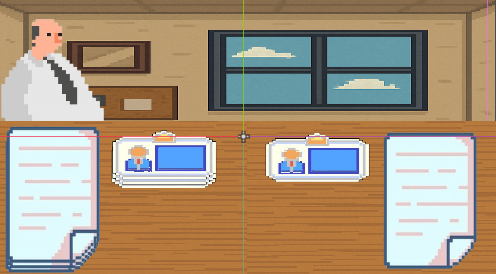
\includegraphics[width=0.6\textwidth]{latex/images/office_concept.png}
    \caption{Általam készített Office munkahely kinézete.}
    \label{fig:office}
\end{figure}

Konkrétan részt vettem az irodai és a Gulag helyszínek textúráinak kidolgozásában, beleértve a háttérképeket, karakterekhez és objektumokhoz tartozó grafikai elemeket, valamint a HUD és menürendszer vizuális elemeit. A textúrákat a Godot projekten belül a megfelelő \texttt{.tscn} kiterjesztésű fájlokban tárolt jelenetekhez társítottam, figyelve a mappastruktúrára és a könnyű integrációra.

\begin{figure}[h]
    \centering
    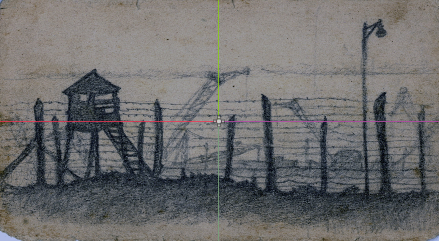
\includegraphics[width=0.6\textwidth]{latex/images/gulag_concept.png}
    \caption{Általam készített gulag concept art.}
    \label{fig:gulag}
\end{figure}

A folyamat során folyamatosan egyeztettünk a csapattagokkal, hogy az elkészült textúrák megfeleljenek az előzetesen kialakított grafikai koncepciónak, valamint biztosítottam a hibák és eltérések gyors javítását. Az elkészült textúrák finomhangolásával a játék vizuális összhatása egységes és koherens lett, amely alapot adott a további fejlesztéshez és a játszható prototípus létrehozásához.

\subsection{Szkriptelés}

A játék szkriptelését elsősorban három fő fájl elkészítésével valósítottam meg: \texttt{game}, \texttt{player} és \texttt{family}.

\begin{itemize}
    \item \textbf{game.gd:} Ez a játék fő vezérlő fájlja, amely inicializálja a karaktereket, betölti a felhasználói felületet (UI) és a HUD-ot, valamint kezeli a különböző játékállapotokat és a scene váltásokat. A játékos (\texttt{Player}) és a családtagok (\texttt{Family}) példányainak létrehozása itt történik, továbbá a HUD frissítése a karakterek aktuális állapotával. Az input események (pl. billentyűleütések) kezelése szintén itt valósul meg.
    \begin{python}
    # UI loading
	var ui_scene = ui.instantiate()
	add_child(ui_scene)
	ui_scene.connect("scene_change_requested",
    Callable(self,"_change_scene"))

    # Scene changing function
    func _change_scene(path: String) -> void:
	   # old scene deleting
	   if current_scene:
		  current_scene.queue_free()
	   # loading
	   var res = load(path)
	   if res:
		  current_scene = res.instantiate()
		  add_child(current_scene)
	   else:
		  push_error("Nem található a scene: %s" % path)
    \end{python}
    \item \textbf{player.gd:} Ez a konstruktor osztály a játékos adatait kezeli. A főbb attribútumok közé tartozik az alkoholszint, éhség, stressz, reputáció, pénz, valamint a rendelkezésre álló tárgyak (pl. kenyér, vodka). Getter és setter függvények biztosítják az adatok lekérését és módosítását, a toString függvény pedig összefoglalja a játékos állapotát egy string formátumban.
    \begin{python}
    # Constructor
    func _init(p_name: String, p_alcohol: int, p_hunger: int,
    p_stress: int, p_reputation: int, p_money: int, p_bread: etc.):
    	player_name = p_name
    	alcohol = p_alcohol
    	hunger = p_hunger
    	stress = p_stress
    	reputation = p_reputation
    	money = p_money
    	bread = p_bread
    	vodka = p_vodka
    # Getters
    func get_player_name() -> String:
	   return player_name
    \end{python}
    \item \textbf{family.gd:} Ez az osztály a családtagok adatait kezeli, például nevüket és éhségüket. Szintén rendelkezik getter és setter függvényekkel, valamint egy toString függvénnyel, amely visszaadja a családtag aktuális állapotát.
    \begin{python}
    # Family data
    var family_member_name: String
    var hunger: int
    # Constructor
    func _init(name: String, h: int):
	   family_member_name = name
	   hunger = h
    # Getters
    func get_family_member_name() -> String:
	   return family_member_name
    func get_hunger() -> int:
	   return hunger
    \end{python}
\end{itemize}

Ezen szkriptfájlok segítségével a játék objektum-orientált módon kezeli a karaktereket és azok interakcióit, lehetővé téve a játék logikájának moduláris, átlátható és könnyen bővíthető felépítését. A \texttt{game.gd} fájlban történik a scene-ek közötti váltás, az UI és HUD integráció, valamint az alap játékmeneti ciklusok vezérlése.

\section{Tesztelés}

A projekt során a \emph{Godot GUT} (Godot Unit Testing) \cite{godot_gut} keretrendszert használtam az egységtesztek és integrációs tesztek elkészítésére. Én elsősorban a következő területeken írtam teszteket:

\begin{itemize}
    \item Irodai animációk és karaktermozgások helyes működésének ellenőrzése.
    \begin{python}
    func before_each():
	main_node = MainNode.new()
	add_child(main_node)

	# --- Mock Boss ---
	var boss = Node2D.new()
	boss.name = "Boss"
	var sprite = AnimatedSprite2D.new()
	sprite.name = "AnimatedSprite2D"
	boss.add_child(sprite)
	main_node.add_child(boss)
	main_node.boss = boss

	# --- Mock Paper & Idcard ---
	var paper = Node2D.new()
	paper.name = "Paper"
	main_node.add_child(paper)
	main_node.paper = paper
    \end{python}
    \item A felhasználói felület (UI) egyes elemeinek, például gombok és menük interakcióinak tesztelése.
    \begin{python}
    # --- Mock Text Layer & Label ---
	var text_layer = CanvasLayer.new()
	text_layer.name = "Text"
	var label = Label.new()
	label.name = "Label"
	text_layer.add_child(label)
	main_node.add_child(text_layer)
	main_node.text_layer = text_layer
	main_node.message_label = label

	# --- Mock UI node ---
	var ui_node = Node.new()
	ui_node.name = "UI"
	main_node.add_child(ui_node)
	main_node.ui = ui_node
    \end{python}
    \item A \texttt{game.gd} fő vezérlő osztály, valamint a konstruktor osztályok (\texttt{player.gd}, \texttt{family.gd}) logikájának validálása.
    \begin{python}
    const Player = preload("res://scripts/player.gd")
    func test_description():
    	var piotr = Player.new("props")
    	
    	# get_description test
    	var desc = piotr.get_description()
    	assert_eq
        (desc, "Player: Piotr | Alcohol: 100 | Hunger: 0 |
        Stress: 0 | Reputation: 50 | Money: 200 | Bread: 5 | 
        Vodka: 2")
    func test_getters():
    	var piotr = Player.new("props")
    	# Getter tests
    	assert_eq(piotr.get_player_name(), "Piotr")
    	assert_eq(piotr.get_alcohol(), 100)
    	assert_eq(piotr.get_hunger(), 0)
    	assert_eq(piotr.get_stress(), 0)
    	assert_eq(piotr.get_reputation(), 50)
    	assert_eq(piotr.get_money(), 200)
    	assert_eq(piotr.get_bread(), 5)
    	assert_eq(piotr.get_vodka(), 2)
    \end{python}
\end{itemize}

A tesztek célja a játék logikájának stabilitásának biztosítása és a különböző komponensek helyes együttműködésének ellenőrzése volt. Különösen az integrációs tesztekkel biztosítottam a HUD, az UI és a játék logikájának összhangját, míg az egységtesztekkel a karakterek és családtagok attribútumainak helyes működését validáltam. \cite{godot_gut}

A tesztelési folyamat során a GitHub repository-ban a pull requestekhez kapcsolódó automatizált tesztek lehetővé tették a hibák korai észlelését és a fejlesztés gyors iterációját.


\section{Összegzés}

A projekt során számos új készséget sajátítottam el és tapasztalatot szereztem a játékfejlesztés különböző területein. Elsősorban a projektmenedzselés, dokumentálás, programozás, textúrázás és tesztelés terén fejlődtem jelentősen. 

A projektmenedzselés során megtanultam a kisebb csapat irányítását, a feladatok hatékony elosztását és nyomon követését, a határidők menedzselését, valamint a kommunikáció és együttműködés koordinálását a csapattagok és a gyakorlatvezető között. Megtanultam, hogyan lehet rugalmasan reagálni a felmerülő problémákra és javaslatokra, miközben fenntartom a projekt folyamatosságát.

A dokumentálás során megtapasztaltam a strukturált, naprakész és egységes dokumentáció fontosságát. Elkészítettem és karbantartottam a projekttervet, az analízis modellt, az SRS dokumentum részeit, a Gantt-diagramokat és a fejlesztési terv részletes heti bontását. Megtanultam, hogyan lehet a dokumentumokat úgy összeállítani, hogy minden csapattag számára világos és könnyen követhető legyen a munkafolyamat.

A programozás terén a Godot Engine és a GDScript használatát sajátítottam el. Megterveztem és implementáltam a játék fő scriptjeit, a \texttt{game.gd}, \texttt{player.gd} és \texttt{family.gd} fájlokat, valamint moduláris, objektum-orientált struktúrát hoztam létre a karakterek és játékelemek kezelésére. Megtanultam a scene-ek kezelését, az UI és HUD integrációját, az input események kezelését, valamint a játéklogika átlátható felépítését.

A textúrázás során fejlődött a vizuális tervezési képességem: elkészítettem a különböző helyszínekhez tartozó textúrákat, karakter- és objektumgrafikákat, valamint a HUD és menürendszer vizuális elemeit. Megtanultam az egységes vizuális stílus kialakítását és a textúrák mappastruktúrába történő helyes integrálását.

A tesztelés során megtanultam az egység- és integrációs tesztek készítését a \emph{Godot GUT} keretrendszer segítségével. Teszteltem a karakterek attribútumait, a UI elemeit, a HUD frissítéseket, valamint a fő játékmeneti ciklusok és konstruktor osztályok működését. Ezáltal fejlődött a hibakeresési és validációs képességem, valamint a stabil és megbízható játéklogika biztosításának tudása.

Összességében a projekt során szerzett tapasztalatok és készségek jelentősen bővítették a technikai, projektmenedzseri és dokumentációs kompetenciáimat. Megtanultam, hogyan lehet egy kisebb csapatot koordinálni, modulárisan felépíteni egy játékot, vizuálisan és logikailag is egységes projektet létrehozni, valamint a fejlesztési folyamatot teszteléssel és dokumentációval támogatni. Mindez megalapozza a további játékfejlesztési és szoftverfejlesztési munkáimat, és magabiztosságot adott a komplex projektek önálló kezeléséhez.

\clearpage

\addcontentsline{toc}{section}{Hivatkozások}
\bibliographystyle{plain}
\bibliography{beszamolo}

\newpage

\include{cover/hasznalati}

\end{document}
